%%%%%%%%%%%%%%%%%%%%%%%%%%%%%%%%%%%%%%%%%%%%%%%%%%%%%%%%%%%%%%%%%%%%%%%%% 
% $Id$
% %%%%%%%%%%%%%%%%%%%%%%%%%%%%%%%%%%%%%%%%%%%%%%%%%%%%%%%%%%%%%%%%%%%%%%%%%
%
% Set de slides sobre el caso de incidencia oblicua
%
% %%%%%%%%%%%%%%%%%%%%%%%%%%%%%%%%%%%%%%%%%%%%%%%%%%%%%%%%%%%%%%%%%%%%%%%%%

  \begin{frame}[allowframebreaks]{Oblique Incidence}

  \begin{columns}
    \column{0.3\textwidth} \centering
    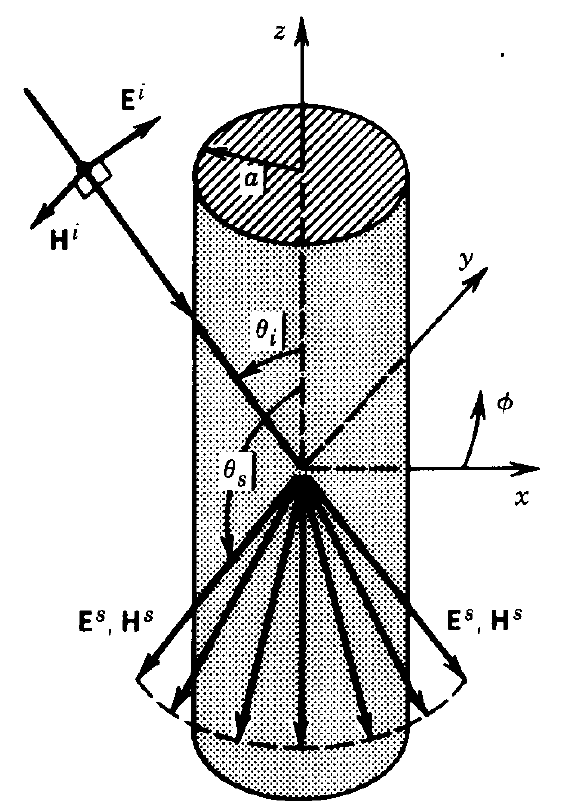
\includegraphics[angle=0,width=\textwidth]{RCS_cylinder_oblique_setup}
    % figure 11.16 Balanis
    % \footnotesize{}
    
    \column{0.65\textwidth} \centering
   \begin{block}{Green Function}
     % \begin{itemize}
     % \item For any  $\theta_i$ we have
       \begin{multline*}
         G = \int_{-\infty}^{\infty} 
        \dfrac{e^{-j k \sqrt{\rho^2+z^2}}}{4\pi \sqrt{\rho^2+z^2}}
        \, e^{\pm j\beta_z z } \, dz \\
        = 
        \begin{cases}
          \dfrac{1}{4j} H_0^{(2)}\left( \rho\sqrt{k^2-\beta_z^2}\right) 
                  & \alert{k^2 > \beta_z^2} \\[2ex]
          \dfrac{1}{2\pi} K_0^{(2)}\left( \rho\sqrt{k^2-\beta_z^2}\right) 
                  & \beta_z^2 > k^2
        \end{cases}
      \end{multline*}
      where $\beta_z^2=k^2\cos^2\theta_i < k^2$

    % \item For $\theta_i=90^\circ$ (normal incidence) we have
    %   $\beta_z=0$ and hence
    %   \begin{equation*}
    %     G = \dfrac{1}{4j} H_0^{(2)}(k|\rho|)
    %   \end{equation*}

    % \end{itemize}
    \end{block}

  \end{columns}


    \framebreak % %%%%%%%%%%%%%%%%%%%%%%%%%%%%%%%%%%%%%%

  \begin{columns}
    \column{0.3\textwidth} \centering
    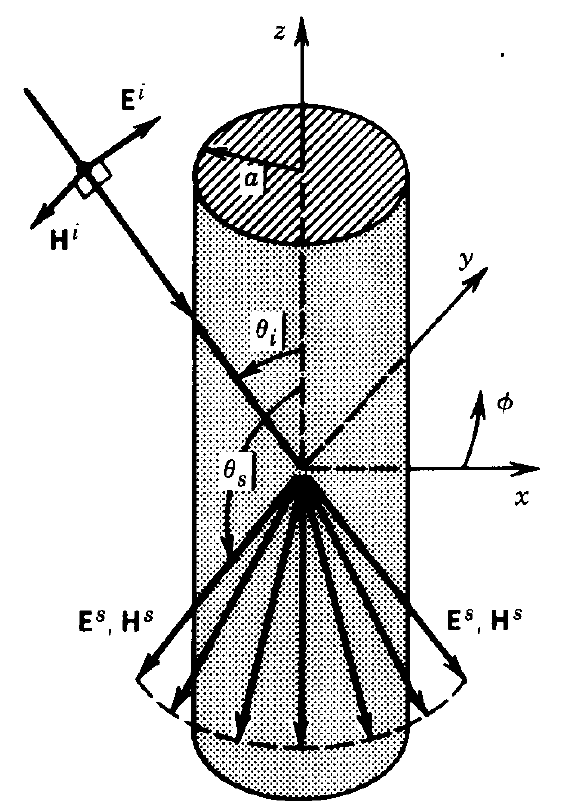
\includegraphics[angle=0,width=\textwidth]{RCS_cylinder_oblique_setup}
    % figure 11.16 Balanis
    % \footnotesize{}
    
    \column{0.65\textwidth} \centering
    \begin{block}{Green Function}
      \begin{itemize}
      \item For any  $\theta_i$ we have
        \begin{equation*}
          G = \dfrac{1}{4j} H_0^{(2)}\left( \rho\sqrt{k^2-\beta_z^2}\right) 
          = \dfrac{1}{4j} H_0^{(2)}\left( k|\rho|\sin\theta_i\right)
        \end{equation*}
        %
      where $\beta_z^2=k^2\cos^2\theta_i < k^2$
        
      \item The particularization to $\theta_i=90^\circ$ (normal
        incidence) yields to the well known result
        % 
        \begin{equation*}
          G = \dfrac{1}{4j} H_0^{(2)}(k|\rho|)
        \end{equation*}
        
      \end{itemize}
    \end{block}
  \end{columns}
  
    \framebreak % %%%%%%%%%%%%%%%%%%%%%%%%%%%%%%%%%%%%%%

  % \begin{columns}
  %   \column{0.3\textwidth} \centering
  %   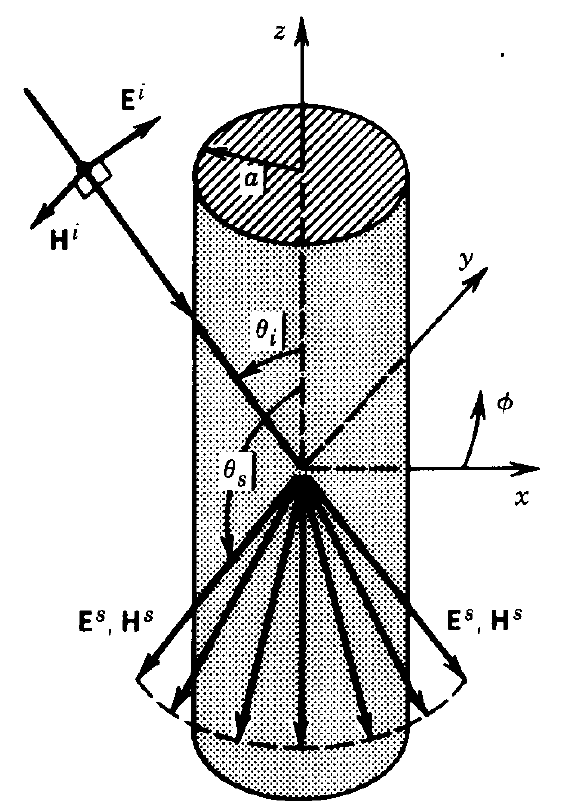
\includegraphics[angle=0,width=\textwidth]{RCS_cylinder_oblique_setup}
  %   % figure 11.16 Balanis
  %   % \footnotesize{}
    
    % \column{0.65\textwidth} \centering
    \begin{block}{FE-IIEE loop}
      \begin{itemize}
      \item As in the case of normal incidence
        \begin{itemize}
        \item We use {\GreenD}\footnote{We may also use {\GreenTEw}}
          on the whole 3D slice and we divide  the scattered field
          at each target point by the ``slice thickness''

        \item We work with $\rho$ instead of $r$, i.e.,
        %
          \begin{equation*}
            |\vrho-\vrhop|=|(\vr-\vrp)-((\vr-\vrp)\cdot\zunit)\zunit|
          \end{equation*}
        %
          where $\zunit$ stands for the direction along the cylinder
          axis\footnote{The code supports arbitrary orientations for the
            cylinder}
        \end{itemize}

      \item The $z$-dependence of the solution (including the scattering field) must be as
        %
        \begin{equation*}
          \vE,\vH \propto   e^{j k \cos\theta_i z} =   e^{-j k \cos\theta_s z}
        \end{equation*}

        Note that $\beta_z=k\cos\theta_i=-k\cos\theta_s>0$
        
      \end{itemize}
    \end{block}

        
    \begin{block}{FE-IIEE loop \insertcontinuationtext}
      \begin{itemize}
      \item Thus, for oblique incidence we need to take into account
        the relative ``height'' between $\vr$ and $\vrp$

      \item That is, we need to add a factor to the 2D Green function
        when summing up the contributions on given integration target
        points of ``height'' $\vr\cdot\zunit$ from different
        integration point sources of ``height'' $\vrp\cdot\zunit$.

        \vbss
        
        The factor is
        % 
        \begin{equation*}
          e^{+j k \cos\theta_i (\vr-\vrp)\cdot\zunit}
          =   e^{-j k \cos\theta_s (\vr-\vrp)\cdot\zunit} 
        \end{equation*}
        %
        or equivalently 
        %
        \begin{equation*}
          e^{-j k \cos\theta_i (\vrp-\vr)\cdot\zunit}
          =   e^{+j k \cos\theta_s (\vrp-\vr)\cdot\zunit}
        \end{equation*}
        % 
        
      \end{itemize}
    \end{block}

    \newpage 
    
    \begin{block}{In other words,}
      
      \begin{equation*}
        G(|\vr-\vrp|) = \dfrac{1}{4j}
        H_0^{(2)}\left( k|\vrho-\vrhop|\sin\theta_i\right) \,
        e^{-j k \cos\theta_i |z-\zp|}
      \end{equation*}

      Remarks:
      \begin{itemize}
      \item Symbol $\zunit$ stands for the direction along the
        cylinder axis
      \item The code supports arbitrary orientations for the cylinder
      \end{itemize}
    \end{block}

    \begin{itemize}
    \item Implementation status:
      \begin{itemize}
      \item Coded
      \item Not tested for oblique cylinder yet (requires PBCs)
      \end{itemize}
    \end{itemize}
      
%  \end{columns}    

    \framebreak % %%%%%%%%%%%%%%%%%%%%%%%%%%%%%%%%%%%%%%

   \large{A remark on dielectric (and dieliectric coated PEC) cylinders\ldots}
    
   \begin{block}{Dielectric cylinders (also dielectric coated PEC)}
     \begin{itemize}
     \item TM and TE are not longer solutions (\alert{polarizations are
       coupled})  for oblique incidence

   \item In the limit, with angle tending to normal incidence, the
     polarizations are effectively decoupled

   \item Analogously, TM and TE coupling appears also when using IBC (even
     isotropic case) for oblique incidence

     \end{itemize}
   \end{block}

  
\end{frame}
  
  % %%%%%%%%%%%%%%%%%%%%%%%%%%%%%%%%%%%%%%%%%%%%%%%%%%%%%%%%%%%%%%%

\begin{frame}[allowframebreaks]{Oblique Incidence}{Far Field
    ---{Update 8 Nov 2022}---}

  \begin{columns}
    \column{0.3\textwidth} \centering
    % AQUI PONER UNA FIGURA MODIFICADA DE ESTA CON SETUP FAR FIELD
   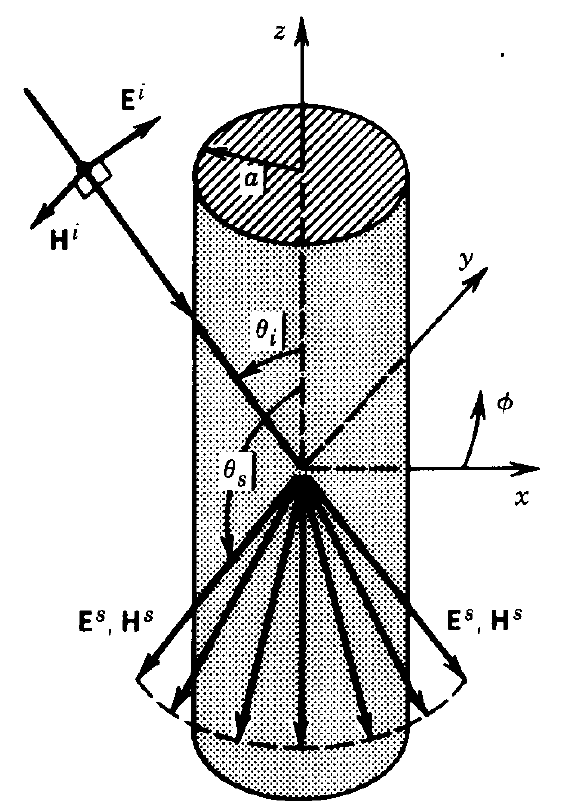
\includegraphics[angle=0,width=\textwidth]{RCS_cylinder_oblique_setup}
    \footnotesize{Far Field Setup}

    
    \column{0.65\textwidth} \centering
   \begin{block}{Far Field }
     \begin{itemize}
     \item Green's function
       \begin{equation*}
        G_\text{far} \propto
        e^{+j k \rho \sin\theta_i}\,
        \underbrace{ e^{-j k \cos\theta_i z}}_{F_{1z}(z)}
      \end{equation*}

    \item Potential, fields
      \begin{equation*}
        \text{Potentials, fields } \propto
        F_{2\phi}(k,\phi,\sin\theta_i) F_{2\theta}(\theta)
      \end{equation*}
      where
      \begin{equation*}
        F_{2\theta}(\theta) = \int_{-\infty}^\infty F_{1z}(z)e^{+j k \cos\theta z}
        = \alert{\delta(\theta-(\pi-\theta_i))}
      \end{equation*}
    \end{itemize}
    \end{block}

  \end{columns}

  \vspace{\baselineskip}
  
%  \begin{itemize}
%  \item
  \centering\parbox{0.9\linewidth}{\alert{Using far field version of {\GreenD} on a 3D
      slice can be used to calculate $F_{2\phi}$ (the variation
      with $\phi$ of the scattering field: RCS, scattering
      width)} % symbol pulgar arriba
  }
    % \item When having a simulato  like HOFEM that uses FE-IIEE loop ....
%  \end{itemize}


  \framebreak % %%%%%%%%%%%%%%%%%%%%%%%%%%%%%%%%%%%%%%
  
  \begin{block}{More precisely\ldots}
    \begin{itemize}
    \item Green's Function 

      \begin{equation*}
        G_\text{far} = \dfrac{1}{4j}
        \left.
          H_0^{(2)}\left( k\rho\sin\theta_i\right)
        \right|_{k\rho\rightarrow\infty} \approx
          \sqrt{\dfrac{2j}{\pi\rho\sin\theta_i}}
        e^{-j k \rho \sin\theta_i}
      \end{equation*}
      
    \end{itemize}

  \end{block}

  \framebreak % %%%%%%%%%%%%%%%%%%%%%%%%%%%%%%%%%%%%%%
  
  \begin{block}{Far Field Computation using 3D Slice}
    \begin{itemize}
    \item We use {\GreenD} on the whole 3D slice and we divide the
      scattered field at each target point by the ``slice thickness''
      
    \item We need to take into account the $z$-dependence of the
      3D (FEM) solution, i.e.,
      % 
      \begin{equation*}
        \vE,\vH \propto   e^{j k \cos\theta_i z}
      \end{equation*}
      
    \end{itemize}

  \end{block}
  
  \framebreak % %%%%%%%%%%%%%%%%%%%%%%%%%%%%%%%%%%%%%%
  
  \begin{block}{Far Field Algorithm:}
  \end{block}
  
    \begin{enumerate}
    \item We start from $\vJ$, $\vM$ on $S'$

    \item We ``equalize'' $\vJ$, $\vM$ on $z$-dependence\footnote{The
        ``equalization'' can alternatively be applied on the Greens's
        Function}
       %
       \begin{align*}
         \vJ &= \vJ \, e^{-j k \cos\theta_i z} \\
         \vM &= \vM \, e^{-j k \cos\theta_i z} 
       \end{align*}

     \item We transform $\vJ$, $\vM$ to spherical coordinates on local
       coordinate system attached to the cylinder
       %
       \begin{align*}
         \vJ &\longrightarrow (J_\theta,J_\phi) \\
         \vM &\longrightarrow (M_\theta,M_\phi) 
       \end{align*}
       
       \begin{itemize}
       \item Note that for normal incidence the local $\theta,\phi$
         components are longitudinal $J_z$, $M_z$ and transverse
         $J_\phi$, $M_\phi$ components, respectively
       \end{itemize}

       \saveenum

    \end{enumerate}


    \framebreak % %%%%%%%%%%%%%%%%%%%%%%%%%%%%%%%%%%%%%%

    
    \begin{enumerate}
      \resumeenum

    \item We compute vector potentials $A_\theta$, $A_\phi$,
      $F_\theta$, $F_\phi$
      %
      \begin{alignat*}{2}
        J_\theta &\rightarrow A_\theta
        & \qquad M_\theta &\longrightarrow F_\theta \\
        J_\phi &\rightarrow A_\phi
        & \qquad M_\phi &\longrightarrow F_\phi
      \end{alignat*}
      

    \item and from vector potentials we compute the far field components
      %
      \begin{equation*}
        (A_\theta,A_\phi,F_\theta,F_\phi) \longrightarrow (E_\theta,E_\phi,H_\theta,H_\phi)
      \end{equation*}

    \item We do not forget to divide by ``slice thickness''
      %
      \begin{equation*}
        (E_\theta,E_\phi,H_\theta,H_\phi) \longrightarrow
             (E_\theta,E_\phi,H_\theta,H_\phi) \, / \, \text{``slice thickness''}
      \end{equation*}
      
    \item Due to decomposition of currents in \alert{local} $\theta$ and $\phi$
      components, we can \alert{naturally obtain the TM and TE components}, i.e.,
      %
      \begin{align*}
        (E_\theta,H_\phi) &\longrightarrow \text{TM} \\
        (E_\phi,H_\theta) &\longrightarrow \text{TE} 
      \end{align*}

    \end{enumerate}
    
    \framebreak % %%%%%%%%%%%%%%%%%%%%%%%%%%%%%%%%%%%%%%

    \begin{block}{Scattering Width $\sigma$}
      \begin{equation*}
        \sigma =
        \begin{bmatrix}
          \sigma_{\text{(TM,TM)}} & \sigma_{\text{(TM,TE)}} \\
          \sigma_{\text{(TE,TM)}} & \sigma_{\text{(TE,TE)}} 
        \end{bmatrix}
      \end{equation*}

      \begin{itemize}
      \item Note that for PEC cylinders we have
        $\sigma_{\text{(TM,TE)}}=\sigma_{\text{(TE,TM)}}=0$
      \end{itemize}
      
    \end{block}


    \vspace{\baselineskip}
   
    
    \begin{itemize}
    \item Implementation status:
      \begin{itemize}
      \item Coded
      \item Not tested for oblique cylinder yet (requires PBCs)
      \end{itemize}
    \end{itemize}
    
\end{frame}
  
% %%%%%%%%%%%%%%%%%%%%%%%%%%%%%%%%%%%%%%%%%%%%%%%%%%%%%%%%%%%%%%%

\begin{frame}[fragile,allowframebreaks]{Integration EMULATION\_2D and PBCs}{Far Field}

  \begin{block}{Logic for Oblique Incidence
      ---\alert{In progress
        (barely initiated)}---}
    \begin{itemize}
    \item \verb|cylinder_axis| and \verb|slice_thickness| obtained  from
      PBC module

    \item Angle of incidence set up in file \url{.em}
      \begin{itemize}
      \item Discard PBC info in file \url{.em}:
        \verb|periodic_phi_angle|, \verb|periodic_theta_angle|
      \item PBC $\longleftarrow$ EMULATION\_2D info from file
        \begin{itemize}
        \item Example: \verb|EMULATION_2D_exterior_angles_1 = {45,140}|
        \end{itemize}
      \end{itemize}

    \item Normal incidence can be run as a particular case
    \end{itemize}
  \end{block}
  

%  REMARK: 
  \begin{itemize}
  \item If \verb|enabled_normal_incidence| there is no PBC interaction (\alert{coded and working})
    \begin{itemize}
    \item \verb|cylinder_axis| and \verb|slice_thickness| read from
      file \url{.em}\footnote{Nevertheless, that information could be
        obtained by preprocessing the mesh within HOFEM code (extra
        task, not considered at present)}
    \item Angle of incidence set up in file \url{.em}:
      \begin{itemize}
      \item Example: \verb|EMULATION_2D_exterior_angles_1 = {90,140}|
      \end{itemize}
    \end{itemize}
  \end{itemize}

  
\end{frame}

% %%%%%%%%%%%%%%%%%%%%%%%%%%%%%%%%%%%%%%%%%%%%%%%%%%%%%%%%%%%%%%%%%%%%%%%%%
